\documentclass{article}
\usepackage[english]{babel}
\usepackage[utf8]{inputenc}
\usepackage{xcolor}
\usepackage[pdftex]{graphicx}
\usepackage{listings}
\usepackage{amsmath}
\usepackage[a4paper,includeheadfoot,margin=2.54cm]{geometry}
\usepackage{amsfonts}
\usepackage{fancyhdr}
\usepackage{titling}
\usepackage{algorithm}
\usepackage{algpseudocode}
\usepackage{hyperref}
\usepackage[export]{adjustbox}
\usepackage{csquotes}
\usepackage{booktabs}

\pagestyle{fancy}
\fancyhf{}
%\fancyhead[LE,RO]{\theauthor}
\fancyhead[RE,LO]{E4 project : Maximin Affinity Learning of Image Segmentation}
\fancyfoot[CE,CO]{\leftmark}
\fancyfoot[LE,RO]{\thepage}

\usepackage[thinlines]{easytable}

\setlength{\parindent}{0ex}


\title{E4 project : Maximin Affinity Learning of Image Segmentation}
\author{Quentin Garrido, Tiphanie Lamy Verdin, Josselin Lefèvre, Annie Lim}
\date{January 2020}

\begin{document}

\maketitle
\pagebreak
\tableofcontents
\pagebreak


\section{Introduction}

The goal of this project is to implement Maximin Affinity Learning of Image
Segmentation (or MALIS for short) as introduced in~\cite{turaga_maximin_2009}.
It is a method used to obtain an image segmentation that is mainly used on medical
imagery.\\

\begin{figure}[!htbp]
	\centering
	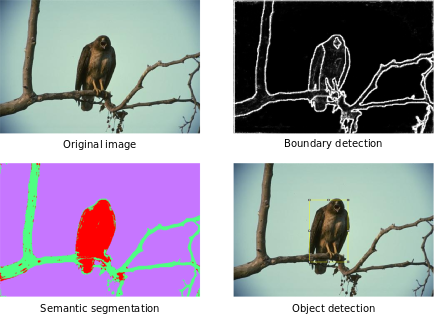
\includegraphics[width=0.7\linewidth]{./images/segmentation.png}
	\caption{Illustration of image segmentation, from
	\href{imagej.net/File:TWS-application-examples.png}{ImageJ}}%
	\label{fig:segmentation}
\end{figure}

As we can see in figure~\ref{fig:segmentation} there are multiple ways to
produce an image segmentation. In the top right corner we can see a boundary
detection of the original image, where borders between objects are in white and
objects are in black. Here we only get the separation between objects but no
information on the objects/segments themselves.\\
In the bottom left corner, we have an example of semantic segmentation of our
image. Here the idea is to classify every pixels in predefined classes (here
red is the bird, green the tree and purple the background). We then obtain a
segmentation with different information, which is not necessarily better than
boundary detection since both solve different problems.\\
On the bottom right corner we have an example of object detection. Even though
it gives us a rough estimate of the structure of the image and the objects
present in it, it is not considered  a segmentation and is a whole other class
of algorithms.\\

In the case of MALIS, we will try to obtain a boundary detection, or what we
could call an edge based segmentation. There are various ways to generate an
image segmentation of this kind, the simplest one being an algorihm such as
Canny's algorithm, or more advanced methods such as watersheds or more recently
neural networks based approaches. The idea with MALIS is to optimize directly a
measure of segmentation quality, which had not been done before. This is a
really interesting idea since segmentations are always evaluated using various
metrics (Rand Index, Variation Of Information ...) and optimizing one directly
could lead to better results, at least for this metric.\\

Our goal in this project is to implement the original MALIS
paper~\cite{turaga_maximin_2009} and also it's improvement
in~\cite{funke_large_2019}.\\

In this report, we will first describe how MALIS works in more details. We will
then look at how we implemented it and some implementation challenges that we
faced. We will then look at the results we have gotten so far, by implementing
the original method. Afterwards, we will look at how the method was improved
and what we will try to implement in the coming semester. Finally we will take
a look at how we worked as a team throughout this project.



%------------------------------------------------------------------------------
\clearpage
\section{Theoretical background}

\input{theory.tex}

%------------------------------------------------------------------------------
\clearpage
\section{Maximin Affinity learning}

\subsection{Method's presentation}

\begin{figure}[!htbp]
	\centering
	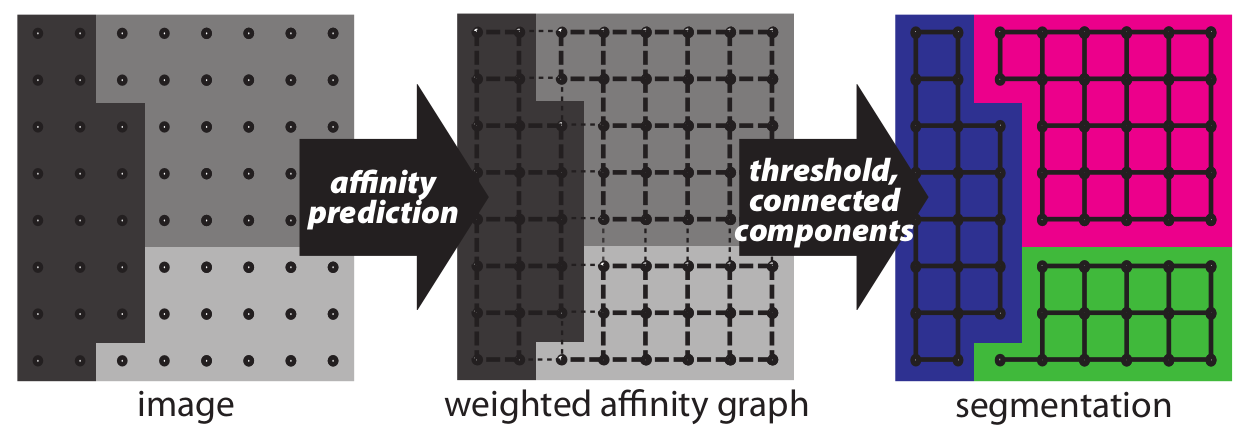
\includegraphics[width=0.8\linewidth]{./images/malis_method.png}
	\caption{Description of the method, from~\cite{turaga_maximin_2009}}%
	\label{fig:malis_method}
\end{figure}

The method, as illustrated in figure~\ref{fig:malis_method} works in two steps.\\
The first step is to compute an affinity graph $G$, with nodes $V$ representing
each pixel in the original image and edges $E$ weighted by the affinity between
neighbouring pixels. The graph $G$ will be 4-connected and for every pair of
pixels $i, j \in V\times V$ there exist and edge $(i,j)\in E$ iff $i$ and $j$ are
neighbours. We will note the affinity between neigbouring pixels $A_{ij}$.\\
An affinity of 1 between $i$ and $j$ means that they belong to the same object,
and an affinity of 0 means that they belong to different objetcs.\\

Once we have our affinity graph, with affinities between 0 and 1, we will
threshold it and remove edges under a certain affinity to obtain connected
components that will be our objects, and this thresholded affinity graph will
be our final segmentation.\\


\subsection{Optimizing the Rand Index}

There exist various methods of evaluating an image segmentation, one of them
being the Rand Index which is defiend as follow :

\begin{gather*}
	1 - RI(\hat{S},S) = \binom{N}{2}^{-1} \sum_{i<j} \lvert \delta(s_i,s_j) -
	\delta(\hat{s}_i,\hat{s}_j) \rvert
\end{gather*}

With $S$ our groundtruth segmentatiin $\hat{S}$ our predicted segmentation and
$\delta(s_i,s_j)$ the indicator function taking value 1 if $s_i = s_j$ (if
pixels $i$ and $j$ are in the same segment/object) and 0 otherwise.\\
Intuitively, this can be seen as the fraction of image pixels where both
segmentations agree.

\begin{figure}[!htbp]
	\centering
	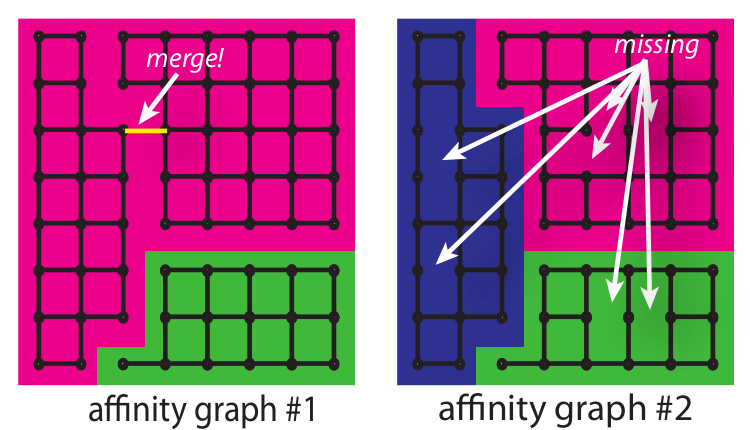
\includegraphics[width=0.45\linewidth]{./images/affinty_graphs.png}
	\caption{Exemple image segmentations and their affinity graph. On the left
	we have a merging of two objects due to a misclassified edge and on the
right we have edges that should be of value 1 that have been removed. From~\cite{turaga_maximin_2009}}%
	\label{fig:affinity_graphs}
\end{figure}

This gives us a way to evaluate an image segmentation that penalizes when two
objects are merged or split in our final segmentation as we can see in
figure~\ref{fig:affinity_graphs}. On the left, only one edge is misclassified
but this merges two objects and will be heavily penalized by the Rand Index (we
would see the same results if an object was split). On the contrary if we have
misclassified edges inside of objects that do not create any splits, this will
not be penalized at all by the loss since our objects are still correctly
delimited.\\

As such the Rand Index seems a good measure of segmentation quality for our
problem (edge-based segmentation). We will have to see how exactly can we
optimise this metric in our case.

\subsection{Maximin affinity and the maximin edge}

In order to optmize the Rand Index, we must find a way to compute
$\delta(\hat{s}_i,\hat{s}_j)$. To to this we will use the concept of maximin
affinity, as described in~\cite{turaga_maximin_2009}.\\
Let $\mathcal{P}_{ij}$ the set of all paths between $i$ and $j$ in our image.
For every path $P\in\mathcal{P}_{ij}$ there is an edge(s) $(k,l)$ with minimal
affinity.\\

This allows us to define the maximin path, which is th path which maximizes the
mininal affinity. It is defined as follow :
\begin{gather*}
	P^*_{ij} =\arg \max_{P\in\mathcal{P}_{ij}}\min_{(k,l)\in P} A_{kl}
\end{gather*}

The edge of minimal affinity in the maximin path will be called the maximin
edge and will be writter $mm(i,j)$.\\
It allows to define the maximin affinity which is simply the affinity of the
maximin edge.
\begin{gather*}
	A^*_{ij} = \max_{P\in\mathcal{P}_{ij}}\min_{(k,l)\in P} A_{kl}
\end{gather*}

The most important consequence of this is that a pair of pixels $i,j$ in connected in
the thresholded affinity graph iff $A^*_{ij}$ is greater than the threshold
value, as shown in~\cite{turaga_maximin_2009}.\\

This means that if we can find the maximin affinity efficiently, we will be
able to compute the Rand Index efficiently.\\
In practice the maximin affinities can bee computed efficiently using a maximum
spanning tree (MST), since any path in the MST is a maximin path.

\subsection{Computing an affinity graph}
As we can see, once we have our affinty graph, obtaining the segmentation is
straightforward, but the issue is : How to obtain an affinity graph? 

As stated before, an affinity graph is equivalent to the contours in the image,
and as such any method to find the contours in an image can be used to find the
affinity graph (with relative success).\\
The first idea that we could have would be to use a contour detector, such as
the Canny filter for example, however this would lead to an obvious over
segmentation, which is not desirable here.\\

An other idea (the idea used in~\cite{turaga_maximin_2009}) would be to use a
neural network to obtain our affinity graph. Neural networks, and particularly
convolutionnal neural networks (CNNs) have proven to be an extremely powerful
tool in image processing and especially in image classification and
segmentation, which makes them a good candidate for MALIS.\\

The architecture used originally is a fully convolutionnal neural network
(FCNN) which is a CNN with only convolutionnal layers. As such they can work
with various input sizes which is always a nice feature.\\

Now that we have seen how we can compute an affinity graph, let's see how we
can train this classifier, and if it even possible to train it with the Rand
Index as a loss function.

\subsection{Training a classifier}

As stated before, the goal of this method is to optimise the Rand Index,
defined as:
\begin{gather*}
	1 - RI(\hat{S},S) = \binom{N}{2}^{-1} \sum_{i<j} \lvert \delta(s_i,s_j) -
	\delta(\hat{s}_i,\hat{s}_j) \rvert
\end{gather*}

with $S$ our groudtruth and $\hat{S}$ our predicted segmentation.\\
We can define $A^*_{ij}(I,\theta)$ the maximin affinity of pixels $i$ and $j$
in the predicted affinty graph of our classifier on $I$ with parameters
$\theta$. We can rewrite the previous equation as :
\begin{gather*}
	1 - RI(I,\theta,S) = \binom{N}{2}^{-1} \sum_{i<j} \lvert \delta(s_i,s_j) -
	 A^*_{ij}(I,\theta)\rvert
\end{gather*}

However this function is not differentiable everywhere so we cannot use it
directly for our training. We will replace the absolute value with a smooth
loss function $l$ such as the mean squared error. This relaxation will allow us
to use gradient descent to train our classifier(refer to~\cite{turaga_maximin_2009}
for more details on this).\\

Thus our final loss function will be :
\begin{gather*}
	L(I,\theta,S) = \binom{N}{2}^{-1} \sum_{i<j} l(\delta(s_i,s_j),
	A^*_{ij}(I,\theta))
	= \binom{N}{2}^{-1} \sum_{i<j} l(\delta(s_i,s_j),A_{mm(i,j)}(I,\theta))
\end{gather*}

We can now look at what the training loop will look like.

\begin{algorithm}
\begin{algorithmic}[1]
\caption{MALIS training loop, from~\cite{turaga_maximin_2009}}\label{alg:malis}
	\Repeat
		\State{Predict the affinity graph for an image $I$}
		\State{Pick two random pixels $i,j$ from $I$}
		\State{Find the maximin edge $mm(i,j)$}
		\State{Update our parameters $\theta$ with gradient}
		\begin{gather*}
			\nabla l(\delta(s_i,s_j),A_{mm(i,j)}(I,\theta)
		\end{gather*}
	\Until{convergence is reached}
\end{algorithmic}
\end{algorithm}

In practice we won't train on the whole image since it would be too long to
compute the maximin edge in the whole image. We will instead train on 21x21
patches of the image. We have to choose these patches carefully as most of them
will mostly be in an object and not around a border.\\
Since borders between objects are far less common than the "inside" of an
object, we may most of the time train only for pixels inside a same object.\\
This would result in class imbalance between our "borders" (affinity of value
0) and or "inside" (affinity of value 1). Training with such imbalance would
lead to worsened results since borders would not be present most of the time in
the chosen image.(one example of such pathological behaviour would be the
prediction of affinty 1 everywhere, far from what we desire)\\

As such when training we need to be careful about what training image we
select.





%------------------------------------------------------------------------------
\clearpage
\section{Implementation}

\subsection{Inputs and outputs of the NN}

After reading the original paper~\cite{turaga_maximin_2009} we realized that
there was some missing information on implementation details.
One of the most important points, the input and the output of the neural
network, was not clear. After some research we were lucky to find Srinivas
Turaga's Phd thesis~\cite{turaga_learning_2010}. In it MALIS was presented in
more details, especially the neural network used in the experiments.\\

The network predicts the affinity following each axis. As we can see in
figure~\ref{fig:nn_output}, in the case where the network is fed a 3D image, it
outputs three affinity images following the axis X, Y and Z. Then we have to
merge these three images in a way to obtain the complete affinity graph.

\begin{figure}[!htbp]
	\centering
	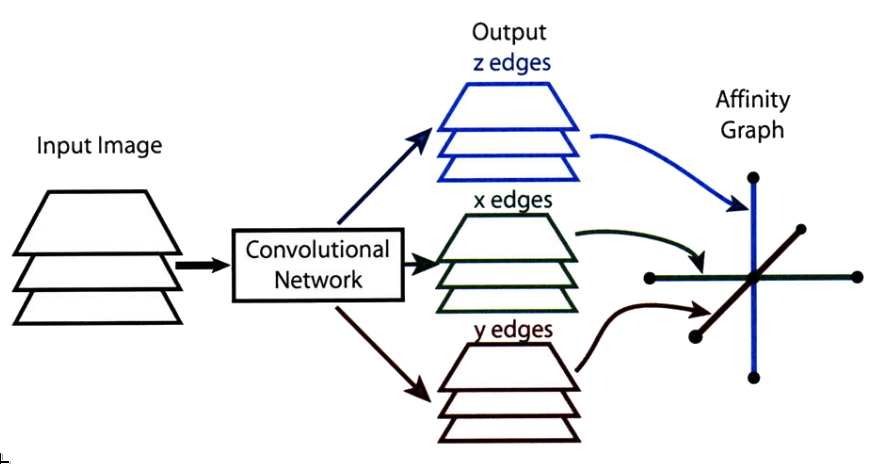
\includegraphics[width=0.8\linewidth]{./images/nn_output.png}
	\caption{Creating the affinity graph using a convolutional network. The
	input to the network is the 3d EM image and the desired output is a set of
3d images: one each for the x, y and z directions representing the affinity
graph, from~\cite{turaga_learning_2010}}%
	\label{fig:nn_output}
\end{figure}

Another problem was to understand the input shape. In the paper, they use a
patch size of $21\times21\times21$. But it is also said that it led to an affinity
classifier that use a patch with a shape of $17\times17\times17$ to classify an affinity
edge. In a first time it was kind of blur but we figured out that 17 correspond
to the volume taking in account after four convolution layers with a kernel
size of $5\times5$, reminiscent to the proposed architecture. The patch size is also arbitrary as we are using a FCN that, by definition, don’t care about the input shape.\\

\subsection{Computing the maximin edge}

As said earlier, we have to find the maximin edge in order to compute the loss.
As we have to do this operation for each training iteration, it is very important to
guarantee a very low computational cost. Our first approach was to use the
Breadth First Search algorithm on the Maximum Spanning Tree efficiently created
with Higra. Sadly, this method was not good because our implementation was
suffering from the slowness of Python and it's $\mathcal{O}(n)$ complexity for each pair of
pixel, which scales badly with the number of pairs chosen. \\

\begin{figure}[!htbp]
	\centering
	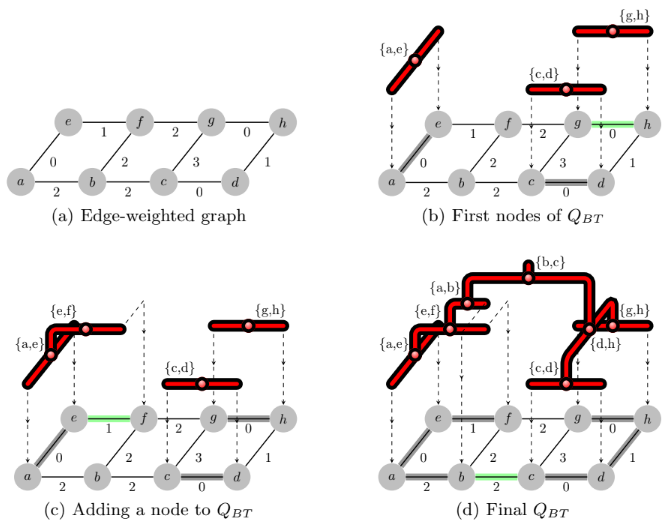
\includegraphics[width=0.7\linewidth]{./images/bpt.png}
	\caption{A simple process for obtaining a binary tree providing a strict
	total order relation on the edges of the MST, from~\cite{najman_playing_2013}}%
	\label{fig:bpt_method}
\end{figure}


In our last version we are computing a Binary Partition Tree, a binary tree by
altitude ordering. This tree is build using Kruskal algorithm. The way to build
this tree is straightforward, as illustrated in figure~\ref{fig:bpt_method}. 
Edges are added to the tree in order of altitude as our MST is built, as
described in \cite{najman_playing_2013}.
This data structure is pretty pertinent as the
maximin edge between to pixel $i$ and $j$ is the lowest common ancestor of these
two pixels in the BPT. Higra also allow us to compute the loss with a larger
number of pairs without an explosion of computing time because picking the
lowest common ancestor is achieved in constant time, with a preprocessing in
$\mathcal{O}(n\log(n))$.

\subsection{Interaction between Higra and PyTorch}

We had some trouble with the interaction between Higra and Pytorch. In order to
compute the loss, we have to compute a BPT on a graph build from the NN output
to find the maximin edge used in the loss computation. As you can see in
figure~\ref{fig:bpt_method}, the gradient history is lost by turning the
affinities images in graph using Higra.\\
We were unable to keep tracking the gradient history by working on
graphs, even after a thorough examination of each step of the process. 
Therefore it was impossible to train our model. But without Higra the
training would be much longer. And even the previous technique using the
Breadth First Search would not work as we are using Higra to compute the MST.
We found the solution in a code proposed by Giovanni Chierchia and Benjamin
Perret in~\cite{chierchia_ultrametric_2019} for computing the subdominant
ultrametric, which is analogous to our problem. Higra has a function that
allow us to make the correspondence between an edge in the graph and the output
affinity image. Consequently, we are able to localise the maximin edge in the
output image. Due to the fact that picking an edge does not cause gradient
history loss we are done.

\begin{figure}[!htbp]
	\centering
	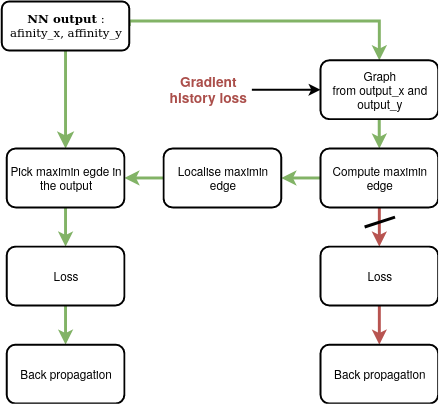
\includegraphics[width=0.6\linewidth]{./images/gradient_history.png}
	\caption{Process to compute the loss from our neural network. The red path
	was our first idea but proved unsuccesful. The green path represents the
process we are using currently.}
	\label{fig:bpt_method}
\end{figure}




%------------------------------------------------------------------------------
\clearpage
\section{Results}

\subsection{Evaluation method}
We evaluated our method with two different datasets : CREMI and ISBI datasets.\\
Both are composed of Drosophila melanogaster adult brain images.\\

Our 3D image of size X x Y x Z was easier to predict in two-dimension. 
That's why we considered Z images of size X x Y which were stacked together to get back a 3D image.\\
A very simple architecture is used for the training.
It's composed of 6 layers of convolution.
In~\ref{turaga_maximin_2009}, the original architecture had 4 layers with 5 features. We decided to add more layers and features to obtain better results. 
Batch normalisations were also added as it didn't exist before.
\begin{center}
	\begin{tabular}{rllllll}\toprule
		Layer & Kernel & Strides & Features & BN &  Activation & Output shape \\
		\midrule
		Input  &  &  & & & & (21, 21, 1)  \\
		Convolution & (5, 5) & (1, 1) & 8 & Y & ReLU  & (21, 21, 8)  \\
		Convolution & (5, 5) & (1, 1) & 32 & Y & ReLU  & (21, 21, 32)  \\
		Convolution & (5, 5) & (1, 1) & 32 & Y & ReLU  & (21, 21, 32)  \\
		Convolution & (5, 5) & (1, 1) & 32 & Y & ReLU  & (21, 21, 32)  \\
		Convolution & (5, 5) & (1, 1) & 8 & Y & ReLU  & (21, 21, 8)  \\
		Convolution & (5, 5) & (1, 1) & 2 & N & sigmoid  & (21, 21, 2)  \\
		\bottomrule
	\end{tabular}
\end{center}

\subsection{CREMI}
The CREMI (Circuit Reconstruction from Electron Microscopy Images) dataset has three volumes but we decided to use only one (volume A) for our training.\\
This 3D image has a size of 1250x1250x125. Its corresponding grountruth was also provided in the dataset. 
The segmentation has labeled connected components with really thin edges.
For the evaluation, we used the CREMI library that was given with the dataset in Python 2. We, then, adapted it in Python 3.\\




A question arises : how to get an image segmentation from the affinity graph ?
We used to different methods to answer this problem.
First of all, a BPT (Binary Partition Tree) and a graph cut could get a good image segmentation. 
However, even with a strong threshold (around 0.99), isthmus appeared and fusion two different objects together.
It's a big issue as it affects our scores.
Secondly, to get rid of isthmus, we did an average affinity.
Isthmus issues can be solved by improving our post-processing, and it should disappear with a better architecture.

Our results are promising as the different objects are well segmented. 
Yet, there are a few oversegmentations when regions are darker. 
Nucleus are not detected as a same object as the cell.

The second volume (volume B) was used as the test set.
The image was similar to the one in the first volume but the objects are more stretched out.
Here the objects are well segmented but it was harder on darker regions.

With more details, we can evaluate with numerical results, according to the Rand index and the VOI (variation of information) merge and split. 
"The Rand index is a measure of the similarity between two data clustering."
*explain VOI*
The Rand index should be the highest as possible, closer to 1. 
The metric VOI should be lower to be better.
In the original architecture of 4 layers, the Rand index is 0.53 while we got 0.61 with our training set and 0.53 with our test set.
Our Rand index is higher to the one of the original architecture.
Our VOI is also lower so better.
Thus, our results are hopeful knowing our architecture used was really simple. 
It's still far from the state of the art but it could get even better with a more complex network.

\subsection{ISBI 2012}






%------------------------------------------------------------------------------
\clearpage
\section{Going forward}


\subsection{Improvement on MALIS}

As we have seen before, MALIS performs really well, but can still be
improved.\\
It was most notably improved in~\cite{funke_large_2019} where they were able to
improve the affinity prediction using more recent architectures, by improving
the training and taking full advantage of the MST and by applying a
post-processing on the affinity graph instead of a simple thresholding.

\begin{figure}[!htbp]
	\centering
	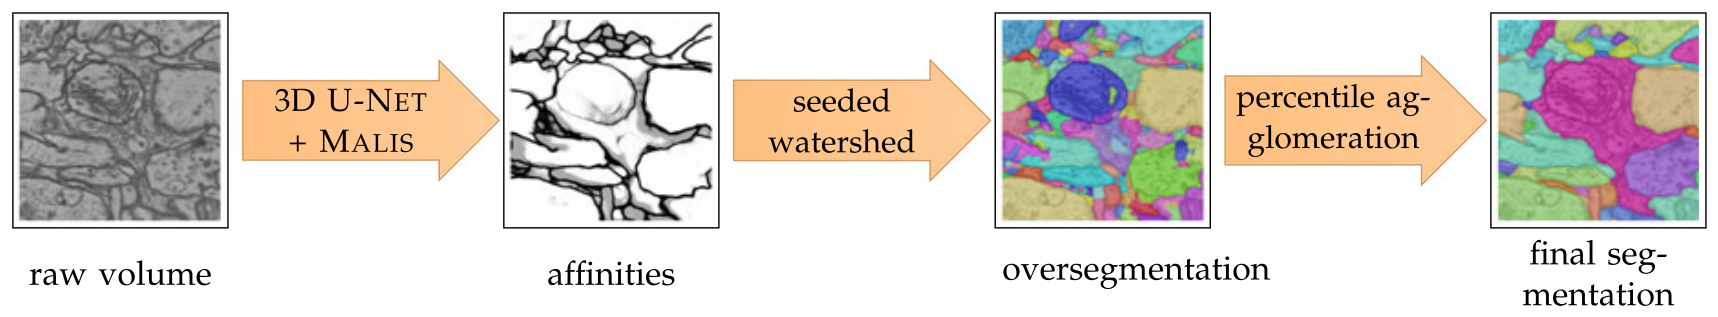
\includegraphics[width=0.8\linewidth]{./images/mala_process.png}
	\caption{Improves MALIS as described in~\cite{funke_large_2019}}%
	\label{fig:mala_process}
\end{figure}

As we can see in figure~\ref{fig:mala_process} the CNN was replaced by a U-Net,
which we will describe afterwards. Then the segmentation is obtained using a
seeded-watershed, which is then improved using a percentile agglomeration of
small objects.

\subsubsection{Using a more potent architecture}
Indeed, one of the limits of the previous method was the use of a relatively
simple neural network to predict the affinity. This is mostly due to the fact
that neural networks have greatly improved since the original
paper~\cite{turaga_maximin_2009} in 2009.\\

\begin{figure}[!htbp]
	\centering
	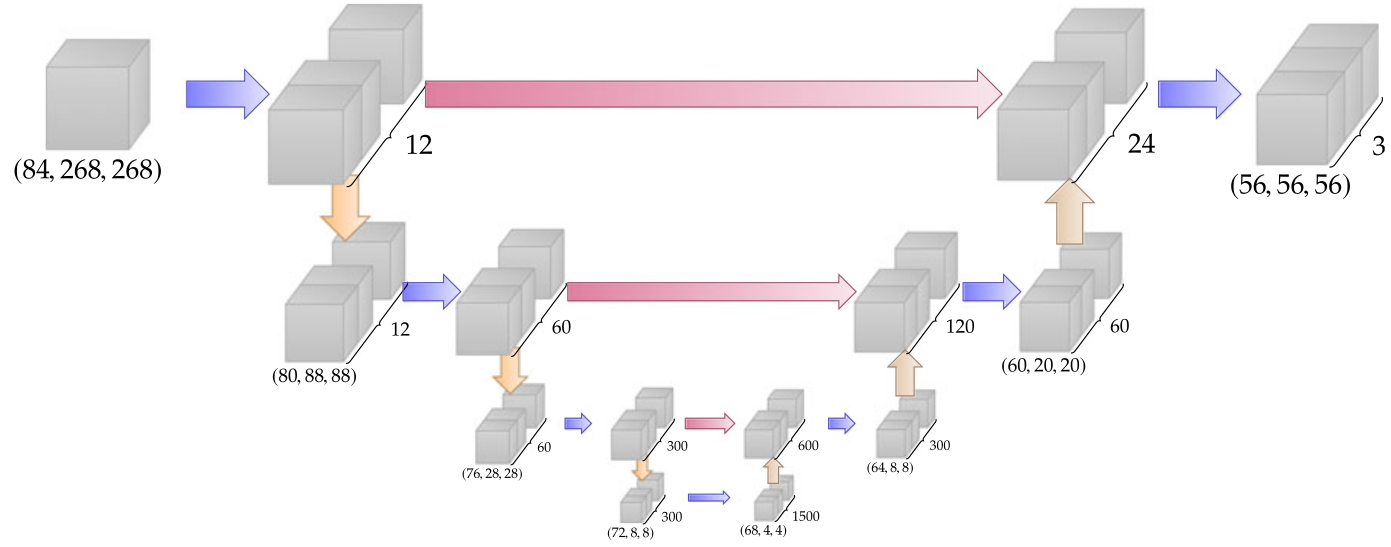
\includegraphics[width=0.8\linewidth]{./images/mala_architecture.png}
	\caption{U-Net architecture used on the CREMI dataset from~\cite{funke_large_2019}}%
	\label{fig:mala_unet}
\end{figure}


U-nets especially have been widely used for image segmentation and are thus a
natural choice in our case. The architecture used in~\cite{funke_large_2019}
is shown in figure~\ref{fig:mala_unet}. As we can see, the training will
obviously be much longer than previously, but the results should be
significantly better.\\
A question that can arise is why not simply use just a U-Net without the MALIS
loss, and as we will see later, the MALIS loss gives us better results on
differents measures of segmentation quality.


\subsubsection{Constrained MALIS loss}

Previously, we only computed the maximin edge for a pair of pixels (or a finite
amount of pairs), which means that some information from the MST was not
used.\\
However, we would like to compute the maximin edge for all pairs of pixels in
the image. This was not done in the previous paper for time efficiency
reasons.\\
However they describe a way to compute the loss with in quasilinear time instead
of in polynomial time.\\

The main idea is that all maximin edges are in the MST, and there are $n-1$
edges if we have $n$ pixels in our image. We could then simply compute the loss
over all those edges but this would mean that they are all as important as the
others. However since we have $n^2$ pairs of points and $n-1$ edges in our MST,
they will be the maximin edge for a different number of pixel-pairs. So we must
find a way to see how often an edge from the MST is a maximin edge.\\

We won't go into much details here on how exactly this is done, but they are
able to find for how many pairs of pixels an edge is a maximin edge when
constructing the MST.\\
When we add an edge using Kruskal's algorithm, we can look at the "size" of the
trees it merges and deduce the number of pairs for which the current edge is
the maximin edge.\\

From this, we can define the positive weight of an edge $e$ as the number of pairs
from the same object/segment merged by adding $e$ to the MST. More formally we
have :
\begin{equation*}
	w_p(e)=\lvert \{(u,v)\in F^2 \;|\;\delta(u,v)=1, e=mm(u,v) \}   \rvert
\end{equation*}

Similarly we can define the negative weight of an edge as :
\begin{equation*}
	w_n(e)=\lvert \{(u,v)\in F^2 \;|\;\delta(u,v)=0, e=mm(u,v) \}   \rvert
\end{equation*}

These formulations allow us to rewrite our loss function as :

\begin{equation*}
	L(I,\theta,S) = \sum_{e\in MST(G)} w_p(e)l(1,A_e(I,\theta)) + w_nl(0,A_e(I,\theta))
\end{equation*}
With $A_e$ the affinity of an edge $e$.\\

With this loss function being able to be computed in quasilinear time, this
will allow us to use the whole patch for the loss computation instead of a few
pairs of pixels, which should improve the results. This loss function is the
same as before, it still is related to the Rand Index, but it should now
approximate it much better.\\


%Vraiment pas convaincu de cette partie
However this doesn't really solve the issue of class imbalance that we noted
before. They suggest a way to resolve this by first computing the positive part
of the loss first (with $w_p$) and then the negative part (with $w_n$). In both
case, we set the other edges (the edges between objects for the positive pass)
to their groundtruth value so that we only take into account a category of
edges.\\
This means that we will computethe loss for edges between objects and edges
inside objects separately, which allows use to combine them afterwards with the
appropriate weights so which should resolve the class imbalance issue.

\subsubsection{Seeded watershed as post processing}

Remember that before, we computed the segmentation by thresholding our affinity
graph. However this doesn't give optimal results, as for example locally
another threshold would perform better.\\
An issue that was also encountered was small objects that were inside bigger
ones. These objects lead to an oversegmentation and we would like a way to
automatically remove those inaccuracies, or at least part of them.

\begin{figure}[!htbp]
	\centering
	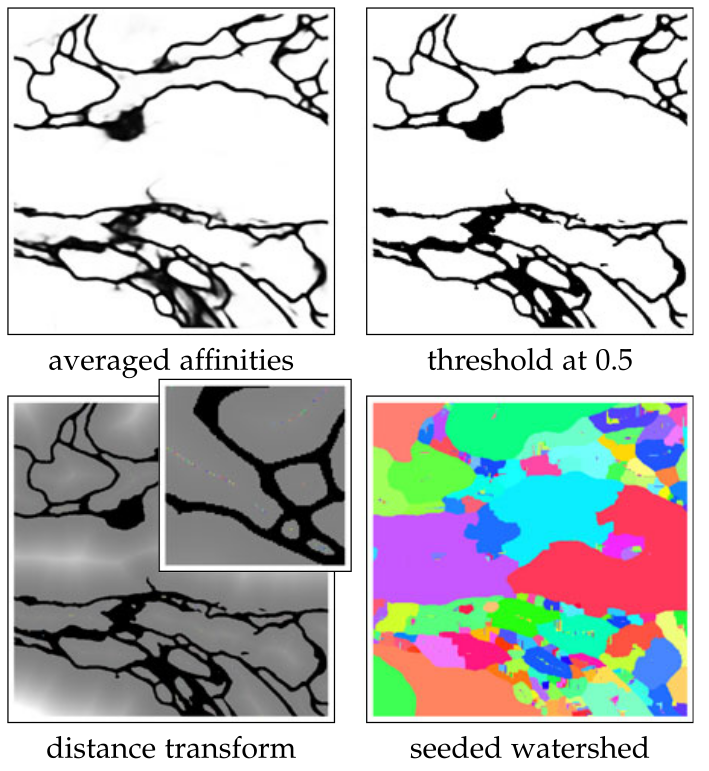
\includegraphics[width=0.5\linewidth]{./images/mala_post_proc.png}
	\caption{Seeded watershed on an affinity graph, as described in~\cite{funke_large_2019}}%
	\label{fig:seeded_ws}
\end{figure}

This is where the framework described in~\cite{funke_large_2019} comes in play.
As we can see in figure~\ref{fig:seeded_ws}, the first step of the process is
to average the affinities, as we did before. Afterwards the averaged affinities
are thresholded at 0.5 (here this threshold is not a parameter). Then a
distance transform (or a distance map) is computed from the objects to the
borders. In this distance transform, the furthest points from the borders will
have the higher values. Then, all the local maxima are taken as seeds for a
seeded watershed, which gives us a first segmentation.\\

This is still an oversegmentation, but a fragment agglomeration algorithm is
then used to fuse regions together. multiple criteria can be used to
determine which regions to merge together and they are described
in~\cite{funke_large_2019}.\\
When all of those steps are done, we obtain the final segmentation.\\

As we can see the process is greatly improved from the first version of MALIS,
with the loss function, the neural network architecture and the post processign
used being much more powerful than their previous counterparts.

\subsection{Goals for the second semester}

The main goal for this next semester will be to implement this improved MALIS.
The mains components to implement are as follow:
\begin{itemize}
	\item Implement the U-Net
	\item Implement the constrained MALIS loss, with it's optimizations
	\item Implement the seeded watershed and fragment agglomeration
	\item Try other methods of post processing
\end{itemize}

Although this is a very important step and a large amount of work, the good
thing with theses improvements is that we can still use parts of the older
method while implementing new ones. For example we can try the U-Net with the
first MALIS loss and no post processing, and the same is true for every new
component that we will implement.\\

Once we have a working implementation the goal will be to try the method on
various datasets. The CREMI dataset will provide us a baseline to compare our
results with those obtained in~\cite{funke_large_2019}. We will also try the
method on other dataset such as the BSDS500 dataset, which is composed of more
varied types of images and not just connectomes.\\

These are our main goals for the second semester, but if we are able to finish
all of this early, there are a lot of interesting experiments where we could
further test the limits of this method.


%------------------------------------------------------------------------------
\clearpage
\section{Teamwork}

\subsection{Team organization}

In order to have an overview of the tasks, we are using the software Trello.
With this, we can write all tasks that we need to do, who is responsible of
the task and the progression of the project: we can see what is already done
and what the other members are currently working on. We communicate with each
other using Slack in which we put information and additional contents related
to the project. \\
Using Trello was really helpful as it always gave us the feeling that we were
progressing, even when we didn't get substantial improvements, we knew that we
had worked and that we were closer to our goal. This helped us stay motivated
at all times.\\

After knowing what tasks we had to do, we split the work based on preferences of
everyone. Quentin was chosen team leader, he worked on a lot of things in the
project and supervised the other team members. Annie worked on the datasets,
both by exploring them and preparing them.
Josselin worked on the computation of the loss and the maximum spanning tree.
Tiphanie worked on the evaluation and the image generation from the output of
our neural network.
We kept everybody informed at all time of what other people did so that
everybody could understand every part of the work.\\

Every week, we had a meeting with our supervisor in which we discussed about
what we did during the week, our issues and solutions if we had some and what
we will do afterwards. During each meeting, a different person lead the
discussion. This helped us improve our communication skills and understanding
of the project as we had to
present both our work and the works others did, and made sure that everybody
spoke for the same amount of time overall. We implemented this since
discussions were almost one-sided before which was not the best solution.\\

We also wrote a report every week in which we wrote what we did in
the week to prepare for the meeting and to show results, or more graphical
elements. We wrote all the codes in documented jupyter notebooks that we will clean and put on GitHub. \\

\subsection{Task distribution}

\begin{table}[!hbtp]
	\centering
	\begin{tabular}{ |p{0.2\linewidth}|p{0.2\linewidth}|p{0.2\linewidth}|p{0.2\linewidth}| } 
		\hline
		Annie & Josselin & Quentin & Tiphanie \\
		\hline
		Find dataset & Computation of MST & Finalize the saliency notebook & Affinity graph thresholding \\ 
		\hline
		Exploration of dataset & Computation and optimisation of the path between i and j & Add features in the saliency notebook & Computation of connected components \\ 
		\hline
		Analyze what is the intput and output of the neural network and their size & Computation of the maximum path in the MST & Graph generation from output of neural network & Image generation \\ 
		\hline
		Understand how to use hdf files & Computation of the loss & Preparation of the dataset & Finishing inference by creating segmentation \\
		\hline
		Create architecture of convolutional neural network & Find interesting patches in dataset & Get vertices pairs in same and different object & Learn PyTorch\\
		\hline
		Load ISBI-2012 data & Train and evaluate on ISBI in 2D & Train the network on maximin affinty & \\
		\hline
		Learn PyTorch & Learn PyTorch & Image reconstruction with inference & \\
		\hline
		  & & Fiji for evaluation on ISBI & \\
		  \hline
		  & & Load ISBI-2012 data & \\
		  \hline
		  & & Train and evaluate on ISBI in 2D & \\
		  \hline
		  & & Learn PyTorch & \\
		  \hline
	\end{tabular}
	\caption{List of the main tasks and their repartition (from our Trello board)}
	\label{tab:tasks}
\end{table}

As we can see in table~\ref{tab:tasks} we tried to distribute the work based on
affinity, and even though the table is unbalanced, everybody put their fair
share of work into the project.\\

One aspect that is absent from this table is all that we learned.
As we will detail in the next section, everybody didn't have the same knowledge
at the beginning of the project and it took everybody a different amount of
time to learn the necessary information.\\

\clearpage
\subsection{Obstacles and overcoming them}

The subject of this project was quite difficult at first because we did not have
any knowledge on image segmentation or morphology. Moreover, it was also hard to read and
understand the scientific papers because they were written in English and
we didn't have the knowledge to understand them clearly at first. To overcome this difficulty, we planned several
hours to go through the important things that we needed to retain, and over
time we were able to grasp more detail from the papers since our knowledge
improved throughout the project.\\

After knowing what we had do, the next step was to figure out how to implement
these ideas.\\
We took some time to know exactly what we needed to do and how to do it in detail for the implementation.
Once we knew, we just needed to find the right functions in Higra.\\
It took us some time to understand how the functions work, as we never used it before.
Documentation is available online and we spent a lot of time learning how to use the
functions.\\
Afterwards, we choose to use the PyTorch library for the deep learning
component of the project, which nobody was familiar with in the group. 
This lack of experience with it meant that we had to spend more time learning
it. However there is a nice tutorial on PyTorch's website that allowed us to
be able to use it fairly quickly. Their documentation on Autograd was also
really helpful when debugging the gradient history loss. Overall the PyTorch
API was really helpful and allowed us to use PyTorch with a relative ease.\\

During this project, we also received a lot of help from Quentin. This project would
have been really hard to do if he was not there, having no great knowledge in
image segmentation and machine learning. Thanks to him, we were able to have a
better understanding of the papers by having him explain them to us. It would have taken us
a lot longer to understand the papers and how to implement them without him and we would 
not be able to present decent results in the end of the first semester presentation.\\

Overall, being aware of the work done by others helped us immensely when
facing issues as we could all think together and challenge each other's
understanding of different topics. This allowed us to overcome all those
difficulties more easily and in a more enjoyable way.


%------------------------------------------------------------------------------
\clearpage
\section{Conclusion}


As we have seen before, even with the implementation of the originak MALIS
paper~\cite{turaga_maximin_2009} we were able to get promising results on both
the CREMI and ISBI datasets.  We were also able to see that the method was greatly
improved in~\cite{funke_large_2019} and this will be the goal that we aim to
reach for the coming semester.\\
We were able to work great as a team and hope that with Raphaël joining us for
this semester we will be able to produce even better results. We also hope that
we will be able to apply the methods to other segmentation tasks, such as the BSDS500 dataset.


\pagebreak
\nocite{*}
\bibliographystyle{ieeetr}
\bibliography{biblio}
\end{document}
